% !TeX spellcheck = en_US
%\documentclass[11pt,a4paper]{article}
\documentclass[11pt
  , a4paper
  , article
  , oneside
%  , twoside
%  , draft
]{memoir}

\usepackage{control}
\usepackage{kotex}
\usepackage[numbers]{natbib}
%\usepackage[pdftex]{graphicx}
%\DeclareGraphicsExtensions{.pdf,.png,.jpg}
\begin{document}

\newcommand{\technumber}{
  Digital Signal Processing using MATLAB}
\title{\textbf{Digital Signal Processing: 실습 12 \\
		제7장 FIR 필터 설계 \\}}

\author{이상일\thanks{silee7103@ibs.re.kr} \\

  학번: 201460437\\
  Computer Engineering, Chungnam National University 
}
\date{\today}

\renewcommand{\maketitlehooka}{\begin{flushright}\textsf{\technumber}\end{flushright}}
%\renewcommand{\maketitlehookb}{\centering\textsf{\subtitle}}
%\renewcommand{\maketitlehookc}{C}
%\renewcommand{\maketitlehookd}{D}

\maketitle

\begin{abstract}
MATLAB을 사용한 Digital Signal Processing에 대한 실습과제에 대한 Documents를 구성한다.
\end{abstract}

\clearpage
\chapter{Example 7-3:}

\begin{lstlisting}[style=termstyle]
% Example 7.3

h = [1,1,1]; w = [0:500]*pi/500;
H = freqz(h,1,w);
magH = abs(H); phaH = angle(H);
ampH = ones(1,501)+2*cos(w); angH = -w;

subplot(2,2,1); plot(w/pi,magH); title('Magnitude Response');
xlabel('frequency in pi units'); ylabel('|H|'); grid
axis([0 1 -1.5 3.5]);

subplot(2,2,3); plot(w/pi,phaH/pi); title('Piecewise Linear Phase Response');
xlabel('frequency in pi units'); ylabel('angle in pi units'); grid
axis([0 1 -1 1])

subplot(2,2,2); plot(w/pi,ampH); title('Amplitude Response');
xlabel('frequency in pi units'); ylabel('Hr'); grid
axis([0 1 -1.5 3.5])

subplot(2,2,4); plot(w/pi,angH/pi); title('Linear Phase Response');
xlabel('frequency in pi units'); ylabel('angle in pi units'); grid
axis([0 1 -1 1])

\end{lstlisting}

\begin{figure}[h!]
	\centering
	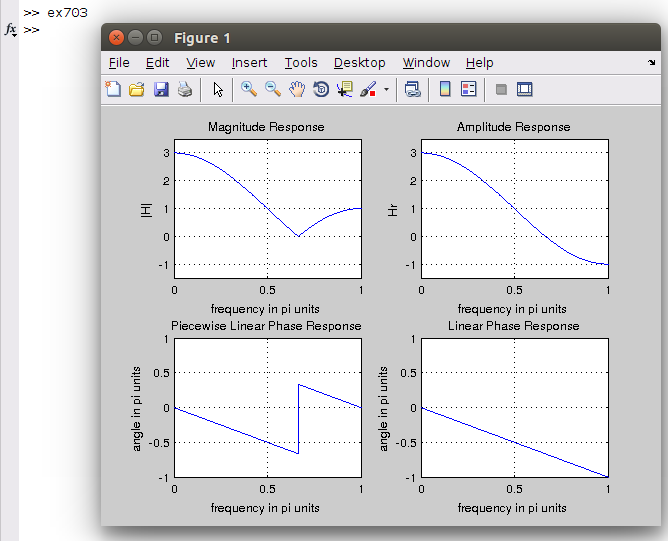
\includegraphics[width=0.6\textwidth,height=0.4\textwidth]{./images/ex703.png}
	\caption{Example 7.3 Result}
	\label{fig:Example 7.3 Result}
\end{figure}

\clearpage
\chapter{Example 7-4:}
\begin{lstlisting}[style=termstyle]
% Example 7.4

h = [-4,1,-1,-2,5,6,5,-2,-1,1,-4];
M = length(h); n = 0:M-1;
[Hr,w,a,L] = Hr_Type1(h);
amax = max(a)+1; amin = min(a)-1;

subplot(2,2,1); stem(n,h); axis([-1 2*L+1 amin amax])
xlabel('n'); ylabel('h(n)'); title('Impulse Response')

subplot(2,2,3); stem(0:L,a); axis([-1 2*L+1 amin amax])
xlabel('n'); ylabel('a(n)'); title('a(n) coefficients')

subplot(2,2,2);plot(w/pi,Hr);grid
xlabel('frequency in pi units'); ylabel('Hr')

title('Type-1 Amplitude Response')
subplot(2,2,4);pzplotz(h,1)

\end{lstlisting}

\begin{figure}[h!]
	\centering
	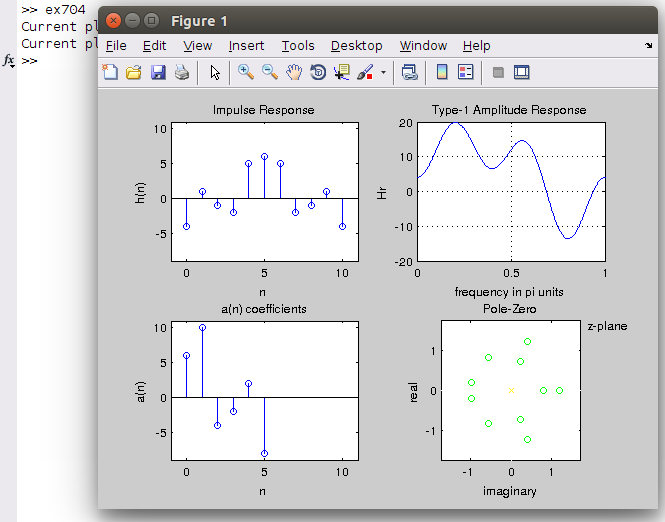
\includegraphics[width=0.6\textwidth,height=0.4\textwidth]{./images/ex704.png}
	\caption{Example 7.4 Result}
	\label{fig:Example 7.4 Result}
\end{figure}

\clearpage
\chapter{Example 7-5:}
\begin{lstlisting}[style=termstyle]
% Example 7.5
h = [-4,1,-1,-2,5,6,6,5,-2,-1,1,-4];
M = length(h); n = 0:M-1;
[Hr,w,b,L] = Hr_Type2(h);
bmax = max(b)+1; bmin = min(b)-1;

subplot(2,2,1); stem(n,h); axis([-1 2*L+1 bmin bmax])
xlabel('n'); ylabel('h(n)'); title('Impulse Response')

subplot(2,2,3); stem(1:L,b); axis([-1 2*L+1 bmin bmax])
xlabel('n'); ylabel('b(n)'); title('b(n) coefficients')

subplot(2,2,2);plot(w/pi,Hr);grid
xlabel('frequency in pi units'); ylabel('Hr')

title('Type-2 Amplitude Response')

subplot(2,2,4);pzplotz(h,1)

\end{lstlisting}

\begin{figure}[h!]
	\centering
	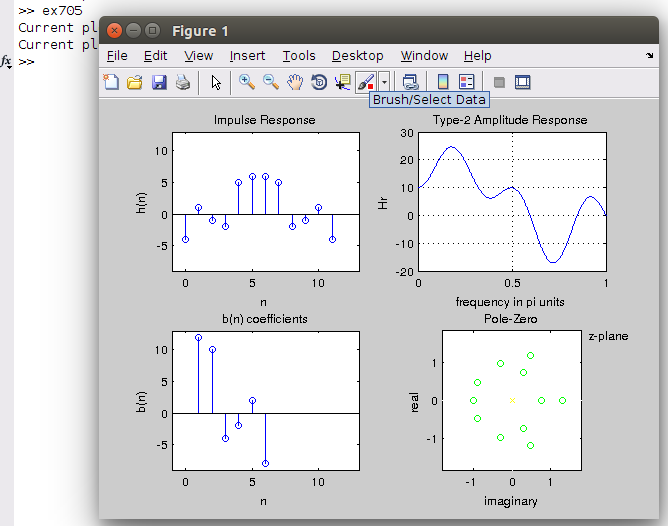
\includegraphics[width=0.6\textwidth,height=0.4\textwidth]{./images/ex705.png}
	\caption{Example 7.5 Result}
	\label{fig:Example 7.5 Result}
\end{figure}

\clearpage

\chapter{Example 7-8:}
\begin{lstlisting}[style=termstyle]
% Example 7.8

wp = 0.2*pi; ws = 0.3*pi;
tr_width = ws - wp
M = ceil(6.6*pi/tr_width) + 1

n=[0:1:M-1];
wc = (ws+wp)/2
hd = ideal_lp(wc,M);
w_ham = (hamming(M))';

h = hd .* w_ham;
[db,mag,pha,grd,w] = freqz_m(h,[1]);
delta_w = 2*pi/1000;
Rp = -(min(db(1:1:wp/delta_w+1)))
As = -round(max(db(ws/delta_w+1:1:501)))

subplot(2,2,1); stem(n,hd); title('Ideal Impulse Response')
axis([0 M-1 -0.1 0.3]); xlabel('n'); ylabel('hd(n)')

subplot(2,2,2); stem(n,w_ham);title('Hamming Window')
axis([0 M-1 0 1.1]); xlabel('n'); ylabel('w(n)')

subplot(2,2,3); stem(n,h);title('Actual Impulse Response')
axis([0 M-1 -0.1 0.3]); xlabel('n'); ylabel('h(n)')

subplot(2,2,4); plot(w/pi,db);title('Magnitude Response in dB');grid
axis([0 1 -100 10]); xlabel('frequency in pi units'); ylabel('Decibels')
\end{lstlisting}

\begin{figure}[h!]
	\centering
	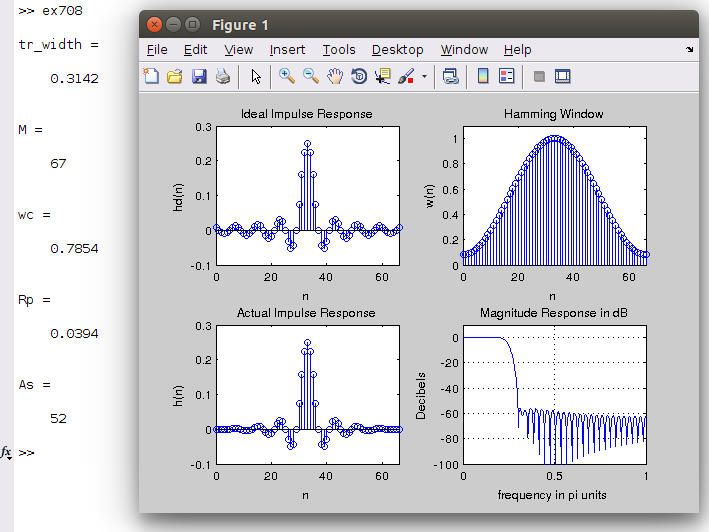
\includegraphics[width=0.6\textwidth,height=0.4\textwidth]{./images/ex708.png}
	\caption{Example 7.8 Result}
	\label{fig:Example 7.8 Result}
\end{figure}

\clearpage
\chapter{Example 7-9:}
\begin{lstlisting}[style=termstyle]
% Example 7.9

wp = 0.2*pi; ws = 0.3*pi; As = 50;
tr_width = ws - wp;
M = ceil((As-7.95)/(14.36*tr_width/(2*pi))+1) + 1

n=[0:1:M-1];
beta = 0.1102*(As-8.7)

wc = (ws+wp)/2;
hd = ideal_lp(wc,M);

w_kai = (kaiser(M,beta))';
h = hd .* w_kai;

[db,mag,pha,grd,w] = freqz_m(h,[1]);
delta_w = 2*pi/1000;
As = -round(max(db(ws/delta_w+1:1:501))) % Min Stopband Attenuation

% Plots
subplot(2,2,1); stem(n,hd); title('Ideal Impulse Response')
axis([0 M-1 -0.1 0.3]); xlabel('n'); ylabel('hd(n)')

subplot(2,2,2); stem(n,w_kai);title('Kaiser Window')
axis([0 M-1 0 1.1]);  xlabel('n'); ylabel('w(n)')

subplot(2,2,3); stem(n,h);title('Actual Impulse Response')
axis([0 M-1 -0.1 0.3]); xlabel('n'); ylabel('h(n)')

subplot(2,2,4);plot(w/pi,db);title('Magnitude Response in dB');grid
axis([0 1 -100 10]); xlabel('frequency in pi units'); ylabel('Decibels')
\end{lstlisting}

\begin{figure}[h!]
	\centering
	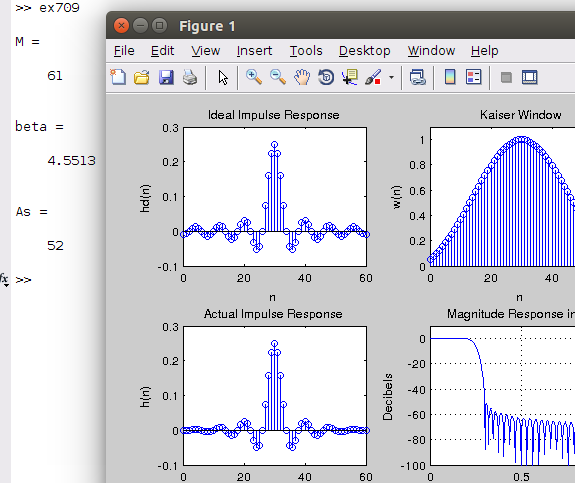
\includegraphics[width=0.6\textwidth,height=0.4\textwidth]{./images/ex709.png}
	\caption{Example 7.9 Result}
	\label{fig:Example 7.9 Result}
\end{figure}

\clearpage
\subsection{Example 7-14}
\begin{lstlisting}[style=termstyle]
% Example 7.14

M = 20; alpha = (M-1)/2; l = 0:M-1; wl = (2*pi/M)*l;
Hrs = [1,1,1,zeros(1,15),1,1];
Hdr = [1,1,0,0]; wdl = [0,0.25,0.25,1];
k1 = 0:floor((M-1)/2); k2 = floor((M-1)/2)+1:M-1;
angH = [-alpha*(2*pi)/M*k1, alpha*(2*pi)/M*(M-k2)];
H = Hrs.*exp(j*angH);
h = real(ifft(H,M));
[db,mag,pha,grd,w] = freqz_m(h,1);
[Hr,ww,a,L] = Hr_Type2(h);

subplot(2,2,1);plot(wl(1:11)/pi,Hrs(1:11),'o',wdl,Hdr); 
axis([0,1,-0.1,1.1]); title('Frequency Samples: M=20')
xlabel('frequency in pi units'); ylabel('Hr(k)')

subplot(2,2,2); stem(l,h); axis([-1,M,-0.1,0.3])
title('Impulse Response'); xlabel('n'); ylabel('h(n)');
subplot(2,2,3); plot(ww/pi,Hr,wl(1:11)/pi,Hrs(1:11),'o');
axis([0,1,-0.2,1.2]); title('Amplitude Response')
xlabel('frequency in pi units'); ylabel('Hr(w)')

subplot(2,2,4);plot(w/pi,db); axis([0,1,-60,10]); grid
title('Magnitude Response'); xlabel('frequency in pi units');
ylabel('Decibels');
\end{lstlisting}

\begin{figure}[h!]
	\centering
	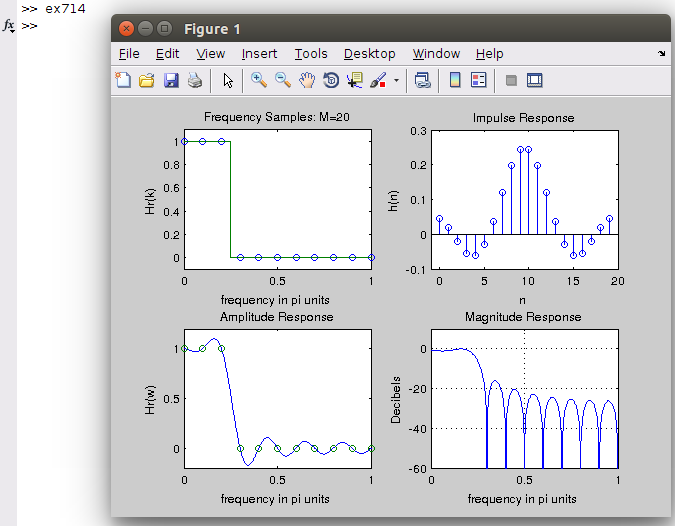
\includegraphics[width=0.5\textwidth,height=0.4\textwidth]{./images/ex714.png}
	\caption{Example 7.14 Result}
	\label{fig:Example 7.14 Result}
\end{figure}

\clearpage
\subsection{Example 7-15a}
\begin{lstlisting}[style=termstyle]
% Example 7.15a
% (a) T1 = 0.5
M = 40; alpha = (M-1)/2; l = 0:M-1; wl = (2*pi/M)*l;
Hrs = [ones(1,5),0.5,zeros(1,29),0.5,ones(1,4)];
Hdr = [1,1,0,0]; wdl = [0,0.25,0.25,1];
k1 = 0:floor((M-1)/2); k2 = floor((M-1)/2)+1:M-1;
angH = [-alpha*(2*pi)/M*k1, alpha*(2*pi)/M*(M-k2)];
H = Hrs.*exp(j*angH);
h = real(ifft(H,M));
[db,mag,pha,grd,w] = freqz_m(h,1);
[Hr,ww,a,L] = Hr_Type2(h);

subplot(2,2,1);plot(wl(1:21)/pi,Hrs(1:21),'o',wdl,Hdr); 
axis([0,1,-0.1,1.1]); title('Frequency Samples: M=40,T1=0.5')
xlabel('frequency in pi units'); ylabel('Hr(k)')

subplot(2,2,2); stem(l,h); axis([-1,M,-0.1,0.3])
title('Impulse Response'); xlabel('n'); ylabel('h(n)');

subplot(2,2,3); plot(ww/pi,Hr,wl(1:21)/pi,Hrs(1:21),'o');
axis([0,1,-0.1,1.1]); title('Amplitude Response')
xlabel('frequency in pi units'); ylabel('Hr(w)')

subplot(2,2,4);plot(w/pi,db); axis([0,1,-100,10]); grid
title('Magnitude Response'); xlabel('frequency in pi units');
ylabel('Decibels');

\end{lstlisting}

\begin{figure}[h!]
	\centering
	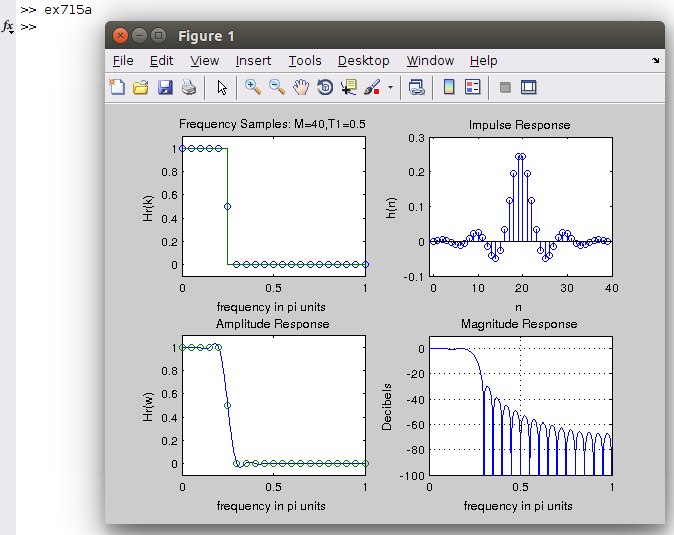
\includegraphics[width=0.5\textwidth,height=0.4\textwidth]{./images/ex715a.png}
	\caption{Example 7.15a Result}
	\label{fig:Example 7.15a Result}
\end{figure}

\clearpage
\subsection{Example 7-15b}
\begin{lstlisting}[style=termstyle]
% Example 7.15b
% (a) T1 = 0.39
M = 40; alpha = (M-1)/2; l = 0:M-1; wl = (2*pi/M)*l;
Hrs = [ones(1,5),0.3904,zeros(1,29),0.3904,ones(1,4)];
Hdr = [1,1,0,0]; wdl = [0,0.25,0.25,1];
k1 = 0:floor((M-1)/2); k2 = floor((M-1)/2)+1:M-1;
angH = [-alpha*(2*pi)/M*k1, alpha*(2*pi)/M*(M-k2)];
H = Hrs.*exp(j*angH);
h = real(ifft(H,M));
[db,mag,pha,grd,w] = freqz_m(h,1);
[Hr,ww,a,L] = Hr_Type2(h);

subplot(2,2,1);plot(wl(1:21)/pi,Hrs(1:21),'o',wdl,Hdr); 
axis([0,1,-0.1,1.1]); title('Frequency Samples: M=40,T1=0.39')
xlabel('frequency in pi units'); ylabel('Hr(k)')

subplot(2,2,2); stem(l,h); axis([-1,M,-0.1,0.3])
title('Impulse Response'); xlabel('n'); ylabel('h(n)');

subplot(2,2,3); plot(ww/pi,Hr,wl(1:21)/pi,Hrs(1:21),'o');
axis([0,1,-0.1,1.1]); title('Amplitude Response')
xlabel('frequency in pi units'); ylabel('Hr(w)')

subplot(2,2,4);plot(w/pi,db); axis([0,1,-100,10]); grid
title('Magnitude Response'); xlabel('frequency in pi units');
ylabel('Decibels');

\end{lstlisting}

\begin{figure}[h!]
	\centering
	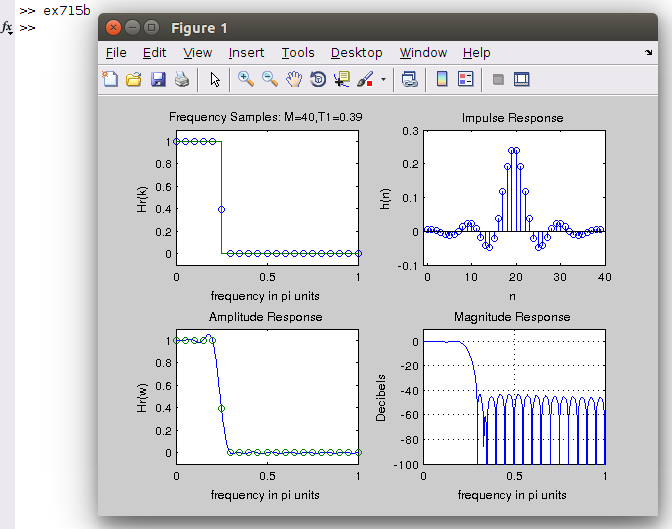
\includegraphics[width=0.5\textwidth,height=0.4\textwidth]{./images/ex715b.png}
	\caption{Example 7.15b Result}
	\label{fig:Example 7.15b Result}
\end{figure}


\clearpage
\subsection{Example 7-16}
\begin{lstlisting}[style=termstyle]
% Example 7.16

M = 60; alpha = (M-1)/2; l = 0:M-1; wl = (2*pi/M)*l;
Hrs = [ones(1,7),0.5925,0.11,zeros(1,43),0.11,0.5925,ones(1,6)];
Hdr = [1,1,0,0]; wdl = [0,0.2,0.3,1];
k1 = 0:floor((M-1)/2); k2 = floor((M-1)/2)+1:M-1;
angH = [-alpha*(2*pi)/M*k1, alpha*(2*pi)/M*(M-k2)];
H = Hrs.*exp(j*angH);
h = real(ifft(H,M));
[db,mag,pha,grd,w] = freqz_m(h,1);
[Hr,ww,a,L] = Hr_Type2(h);

subplot(2,2,1);plot(wl(1:31)/pi,Hrs(1:31),'o',wdl,Hdr); 
axis([0,1,-0.1,1.1]); title('Lowpass: M=60,T1=0.59, T2=0.109')
xlabel('frequency in pi units'); ylabel('Hr(k)')

subplot(2,2,2); stem(l,h); axis([-1,M,-0.1,0.3])
title('Impulse Response'); xlabel('n'); ylabel('h(n)');

subplot(2,2,3); plot(ww/pi,Hr,wl(1:31)/pi,Hrs(1:31),'o');
axis([0,1,-0.1,1.1]); title('Amplitude Response')
xlabel('frequency in pi units'); ylabel('Hr(w)')

subplot(2,2,4);plot(w/pi,db); axis([0,1,-100,10]); grid
title('Magnitude Response'); xlabel('frequency in pi units');
ylabel('Decibels');

\end{lstlisting}

\begin{figure}[h!]
	\centering
	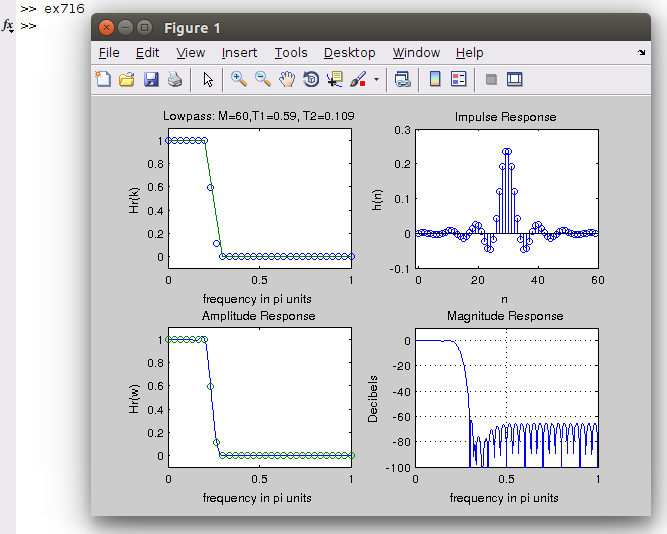
\includegraphics[width=0.5\textwidth,height=0.4\textwidth]{./images/ex716.png}
	\caption{Example 7.16 Result}
	\label{fig:Example 7.16 Result}
\end{figure}


\clearpage
\chapter{Common: M-Functions}
pzplotz.m:
\begin{lstlisting}[style=termstyle]
function pzplotz(b,a)
%  pzplotz(b,a) 
%  b 
%  a
%  a,b
N = length(a); M = length(b); pz = []; zz = []; 
if (N > M)
zz = zeros((N-M),1);
elseif (M > N)
pz = zeros((M-N),1); 
end
pz = [pz;roots(a)]; zz = [zz;roots(b)];
pzr = real(pz)'; pzi = imag(pz)';
zzr = real(zz)'; zzi = imag(zz)';
rzmin = min([pzr,zzr,-1])-0.5; rzmax = max([pzr,zzr,1])+0.5;
izmin = min([pzi,zzi,-1])-0.5; izmax = max([pzi,zzi,1])+0.5;
zmin = min([rzmin,izmin]); zmax = max([rzmax,izmax]); zmm = max(abs([zmin,zmax]));
%
uc=exp(j*2*pi*[0:1:500]/500);
plot(real(uc),imag(uc),'w',[-zmm,zmm],[0,0],'w',[0,0],[-zmm,zmm],'w');
axis([-zmm,zmm,-zmm,zmm]);axis('square');hold
plot(zzr,zzi,'go',pzr,pzi,'yx');hold
text(zmm*1.1,zmm*0.95,'z-plane')
xlabel('imaginary');ylabel('real')
title('Pole-Zero')
\end{lstlisting}

ideal\_lp.m:
\begin{lstlisting}[style=termstyle]
function hd = ideal_lp(wc,M);
% Ideal LowPass filter computation
% [hd] = ideal_lp(wc,M)
%  hd = ideal impulse response between 0 to M-1
%  wc = cutoff frequency in radians
%   M = length of the ideal filter
%
alpha = (M-1)/2;
n = [0:1:(M-1)];
m = n - alpha + eps;
hd = sin(wc*m) ./ (pi*m);
\end{lstlisting}

freqz\_m.m:
\begin{lstlisting}[style=termstyle]
function [db,mag,pha,grd,w] = freqz_m(b,a);
% Modified version of freqz subroutine
% ------------------------------------
% [db,mag,pha,grd,w] = freqz_m(b,a);
%  db = Relative magnitude in dB computed over 0 to pi radians
% mag = absolute magnitude computed over 0 to pi radians 
% pha = Phase response in radians over 0 to pi radians
% grd = Group delay over 0 to pi radians
%   w = 501 frequency samples between 0 to pi radians
%   b = numerator polynomial of H(z)   (for FIR: b=h)
%   a = denominator polynomial of H(z) (for FIR: a=[1])
[H,w] = freqz(b,a,1000,'whole');
H = (H(1:1:501))'; w = (w(1:1:501))';
mag = abs(H);
db = 20*log10((mag+eps)/max(mag));
pha = angle(H);
%  pha = unwrap(angle(H));
grd = grpdelay(b,a,w);
%  grd = diff(pha);
%  grd = [grd(1) grd];
%  grd = [0 grd(1:1:500); grd; grd(2:1:501) 0];
%  grd = median(grd)*500/pi;
\end{lstlisting}


\end{document}

